
%----------------------------------------------------------------------------------------%
% START LaTeX preamble

% define document type, font and paper size
\documentclass[11pt,a4paper]{article}

%----------------------------------------------------------------------------------------%
% IMPORT LaTeX packages

\usepackage{inputenc}
\usepackage[ngerman, english]{babel}
\usepackage{csquotes}
\usepackage{amsmath}
\usepackage{amssymb}
\usepackage{amsfonts}
\usepackage{graphicx}
\usepackage{wrapfig}
\usepackage[margin=1.25in]{geometry}
\usepackage{pdfpages}
\usepackage{listings}
\usepackage{setspace}
\usepackage{systeme}
\usepackage{mdframed}
\newcommand{\mathsym}[1]{{}}
\newcommand{\unicode}[1]{{}}




%----------------------------------------------------------------------------------------%
% IMPORT LaTeX packages to manange bibliography

% MLA, APA, or IEEE? - https://www.overleaf.com/learn/latex/Biblatex_citation_styles
\usepackage[style=apa, backend=biber]{biblatex}
\addbibresource{bibliography.bib}

%----------------------------------------------------------------------------------------%
% DEFINE header values

% define the cover page values
\title
{
    Homework 03 - Matrix Inversion
}
\author
{    
    Bruno Gonz{\' a}lez Soria (A01169284)  \\
    Antonio Osamu Katagiri Tanaka (A01212611) \\
    Jos{\' e} Ivan Aviles Castrillo (A01749804) \\
    Jes{\' u}s Alberto Mart{\' i}nez Espinosa (A01750270) \\
    Katya Michelle Aguilar P{\' e}rez (A01750272) \\
    \\
    Instructor: Ph.D Daniel L{\' o}pez Aguayo
}
\date{\today}

%----------------------------------------------------------------------------------------%
% USER-DEFINED commands

% Keywords command
\providecommand{\keywords}[1]
{
    \\
    \\
    \small
    \textbf{\textit{Keywords:}} #1
}

%----------------------------------------------------------------------------------------%

\begin{document}
\setlength\parindent{0pt} % Set noindent for entire file

%----------------------------------------------------------------------------------------%
% CREATE the 1st page (cover page)

\maketitle

%----------------------------------------------------------------------------------------%
% DEFINE the abstract text & keywords

%\begin{abstract}
%    \emph
%    {
%        Lorem ipsum dolor sit amet, consectetur adipiscing elit, sed do eiusmod tempor incididunt ut labore et dolore magna aliqua. Ut enim ad minim veniam, quis nostrud exercitation ullamco laboris nisi ut aliquip ex ea commodo consequat. Duis aute irure dolor in reprehenderit in voluptate velit esse cillum dolore eu fugiat nulla pariatur. Excepteur sint occaecat cupidatat non proident, sunt in culpa qui officia deserunt mollit anim id est laborum.
%    }
%    \keywords{Lorem, ipsum, dolor, sit, amet}
%\end{abstract}
\clearpage

%----------------------------------------------------------------------------------------%
% CREATE a table of contents in a new page

%\tableofcontents
%\clearpage

%----------------------------------------------------------------------------------------%
% CREATE a list of figures and a list of tables in a new page

%\listoffigures
%\listoftables
%\clearpage

%----------------------------------------------------------------------------------------%
% DOCUMENT body starts here

%----------------------------------------------------------------------------------------%
%Append the HW's exercises
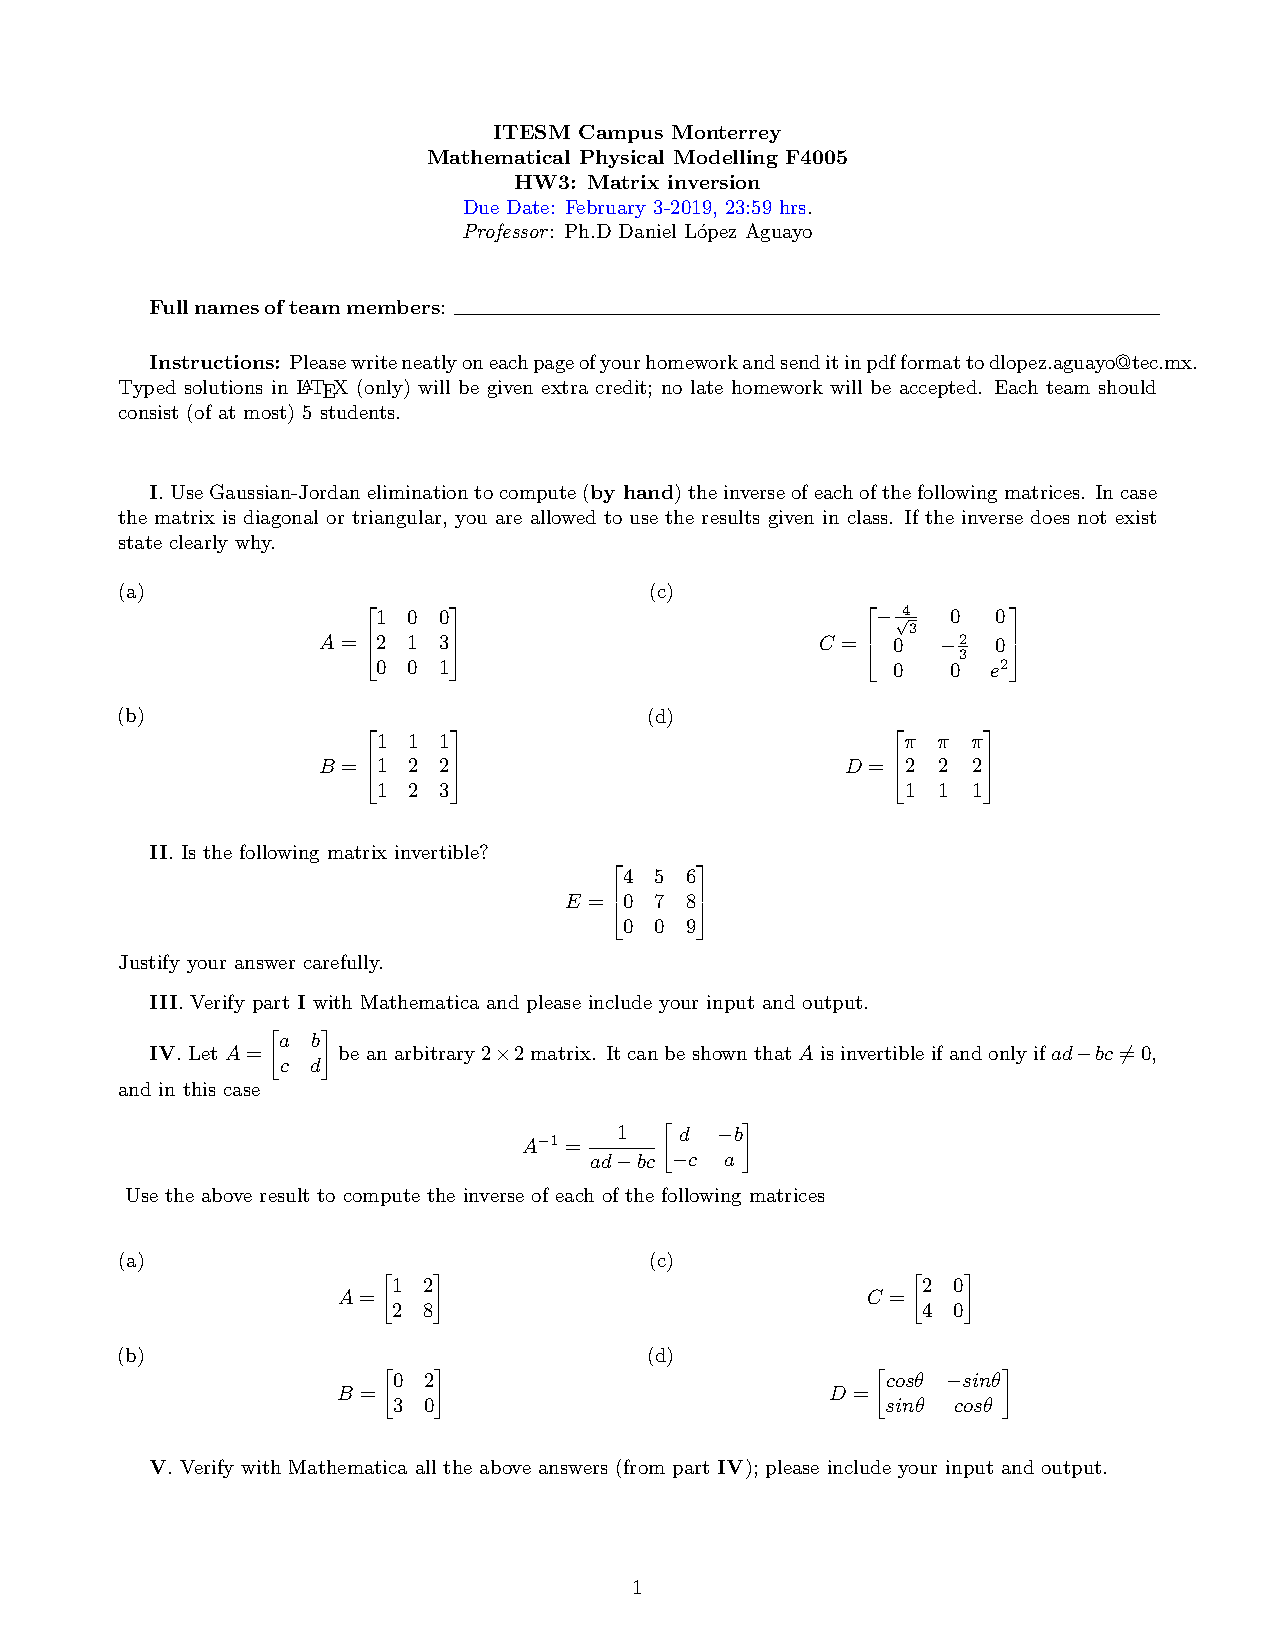
\includepdf[page=-]{HW3}

%----------------------------------------------------------------------------------------%
\section{Answer to Problem I}\label{sec:P01}



\clearpage
%----------------------------------------------------------------------------------------%
\section{Answer to Problem II}\label{sec:P02}



\clearpage
%----------------------------------------------------------------------------------------%
\section{Answer to Problem III}\label{sec:P03} %Osamu

\hfill \break
III.a\\
\begin{doublespace}
\noindent\(\pmb{\text{varA}=\left(
\begin{array}{ccc}
 1 & 0 & 0 \\
 2 & 1 & 3 \\
 0 & 0 & 1 \\
\end{array}
\right);}\\
\pmb{\text{Inverse}[\text{varA}];}\\
\pmb{\text{MatrixForm}[\%]}\)
\end{doublespace}

\begin{doublespace}
\noindent\(\left(
\begin{array}{ccc}
 1 & 0 & 0 \\
 -2 & 1 & -3 \\
 0 & 0 & 1 \\
\end{array}
\right)\)
\end{doublespace}

\hfill \break
III.b\\
Matrix is singular.

\begin{doublespace}
\noindent\(\pmb{\text{varB}=\left(
\begin{array}{ccc}
 1 & 1 & 1 \\
 1 & 2 & 2 \\
 1 & 3 & 3 \\
\end{array}
\right);}\\
\pmb{\text{Inverse}[\text{varB}];}\)
\end{doublespace}

\hfill \break
III.c\\
\begin{doublespace}
\noindent\(\pmb{\text{varC}=\left(
\begin{array}{ccc}
 -\frac{4}{\sqrt{3}} & 0 & 0 \\
 0 & -\frac{2}{3} & 0 \\
 0 & 0 & e^2 \\
\end{array}
\right);}\\
\pmb{\text{Inverse}[\text{varC}];}\\
\pmb{\text{MatrixForm}[\%]}\)
\end{doublespace}

\begin{doublespace}
\noindent\(\left(
\begin{array}{ccc}
 -\frac{\sqrt{3}}{4} & 0 & 0 \\
 0 & -\frac{3}{2} & 0 \\
 0 & 0 & \frac{1}{e^2} \\
\end{array}
\right)\)
\end{doublespace}

\clearpage
\hfill \break
III.d\\
Matrix is singular.

\begin{doublespace}
\noindent\(\pmb{\text{varD}=\left(
\begin{array}{ccc}
 \pi  & \pi  & \pi  \\
 2 & 2 & 2 \\
 1 & 1 & 1 \\
\end{array}
\right);}\\
\pmb{\text{Inverse}[\text{varD}];}\)
\end{doublespace}

\clearpage
%----------------------------------------------------------------------------------------%
\section{Answer to Problem IV}\label{sec:P04} %Osamu

IV.a\\
$
A^{-1}= \frac{1}{1(8)-2(2)}\left(
\begin{array}{cc}
 8 & -2 \\
 -2 & 1 \\
\end{array}
\right)= \frac{1}{4}\left(
\begin{array}{cc}
 8 & -2 \\
 -2 & 1 \\
\end{array}
\right)= \left(
\begin{array}{cc}
 2 & -\frac{1}{2} \\
 -\frac{1}{2} & \frac{1}{4} \\
\end{array}
\right)
$

\hfill \break
IV.b\\
$
B^{-1}= \frac{1}{0(0)-2(3)}\left(
\begin{array}{cc}
 0 & -2 \\
 -3 & 0 \\
\end{array}
\right)= -\frac{1}{6}\left(
\begin{array}{cc}
 0 & -2 \\
 -3 & 0 \\
\end{array}
\right)= \left(
\begin{array}{cc}
 0 & \frac{1}{3} \\
 \frac{1}{2} & 0 \\
\end{array}
\right)
$

\hfill \break
IV.c\\
$
C^{-1}= \frac{1}{2(0)-0(4)}\left(
\begin{array}{cc}
 0 & 0 \\
 -4 & 2 \\
\end{array}
\right)\Rightarrow ad-bc\ is not equal to\ 0,\ therefore\ C^{-1}\ does\ not\ exist.
$

\hfill \break
IV.d\\
$
D^{-1}= \frac{1}{\text{Cos}[\theta ](\text{Cos}[\theta ])-(-\text{Sin}[\theta ])(\text{Sin}[\theta ])}\left(
\begin{array}{cc}
 \text{Cos}[\theta ] & \text{Sin}[\theta ] \\
 -\text{Sin}[\theta ] & \text{Cos}[\theta ] \\
\end{array}
\right)= \frac{1}{\text{Cos}[\theta ]^2+\text{Sin}[\theta ]^2}\left(
\begin{array}{cc}
 \text{Cos}[\theta ] & \text{Sin}[\theta ] \\
 -\text{Sin}[\theta ] & \text{Cos}[\theta ] \\
\end{array}
\right)= \left(
\begin{array}{cc}
 \frac{\text{Cos}[\theta ]}{\text{Cos}[\theta ]^2+\text{Sin}[\theta ]^2} & \frac{\text{Sin}[\theta ]}{\text{Cos}[\theta ]^2+\text{Sin}[\theta ]^2}
\\
 -\frac{\text{Sin}[\theta ]}{\text{Cos}[\theta ]^2+\text{Sin}[\theta ]^2} & \frac{\text{Cos}[\theta ]}{\text{Cos}[\theta ]^2+\text{Sin}[\theta ]^2}
\\
\end{array}
\right)
$

\clearpage
%----------------------------------------------------------------------------------------%
\section{Answer to Problem V}\label{sec:P05} %Osamu

\hfill \break
V.a\\
\begin{doublespace}
\noindent\(\pmb{\text{Custom2by2Inverse}[\text{varM$\_$}]\text{:=}\text{Module}[\{\text{vM}=\text{varM}, a,b,c,d,\text{Res}\},}\\
\pmb{\text{(* }\text{Let}'s \text{ check } \text{if } \text{the } \text{matrix } \text{is } \text{of } \text{size } 2\text{x2 }\text{*)}}\\
\pmb{\text{If}[\text{Dimensions}[\text{vM}][[1]]==2 \&\& \text{Dimensions}[\text{vM}][[2]]==2,}\\
\pmb{a=\text{vM}[[1,1]];}\\
\pmb{b=\text{vM}[[1,2]];}\\
\pmb{c=\text{vM}[[2,1]];}\\
\pmb{d=\text{vM}[[2,2]];}\\
\pmb{\text{(* }\text{The } \text{matrix } \text{is } \text{invertible } \text{if } \text{and } \text{only } \text{if } \text{ad}-\text{bc}\neq 0 \text{ ... }\text{*)}}\\
\pmb{\text{If}[a*d-b*c==0,}\\
\pmb{\text{Print}[\text{{``}[ERROR] The matrix is not invertible.{''}}]}\\
\pmb{];}\\
\pmb{\text{(* Use the provided equation to calculate the inverse of the 2x2 matrix *)}}\\
\pmb{\text{Res}=\frac{1}{a*d-b*c}\left(
\begin{array}{cc}
 d & -b \\
 -c & a \\
\end{array}
\right);}\\
\pmb{\text{(* }\text{Use } \text{Mathematica}'s \text{ function } \text{Inverse}[] \text{ to } \text{verify } \text{the } \text{calculation }\text{*)}}\\
\pmb{\text{If}[\text{Res}==\text{Inverse}[\text{varM}],}\\
\pmb{\text{Print}[\text{{``}[PASS] The calculation is EQUAL to Mathematica's function Inverse[{''}},}\\
\pmb{\text{MatrixForm}[\text{varM}],\text{{``}].{''}}],}\\
\pmb{\text{Print}[\text{{``}[FAIL] The calculation is NOT EQUAL to Mathematica's function Inverse[{''}},}\\
\pmb{\text{MatrixForm}[\text{varM}],\text{{``}].{''}}]}\\
\pmb{];}\\
\pmb{\text{(*Return the calculated inverse of vM*)}}\\
\pmb{\text{Res},}\\
\pmb{\text{(*Display an error message if the matrix size is not 2x2*)}}\\
\pmb{\text{Print}(\text{{``}[ERROR] Unfortunately, this function only works with 2x2 matrices.{''}})}\\
\pmb{];}\\
\pmb{];}\\
\pmb{\text{Custom2by2Inverse}\left[\left(
\begin{array}{cc}
 1 & 2 \\
 2 & 8 \\
\end{array}
\right)\right];}\\
\pmb{\text{MatrixForm}[\%]}\)
\end{doublespace}

\noindent\(\text{[PASS] The calculation is EQUAL to Mathematica's function Inverse[}\left(
\begin{array}{cc}
 1 & 2 \\
 2 & 8 \\
\end{array}
\right)\text{].}\)

\begin{doublespace}
\noindent\(\left(
\begin{array}{cc}
 2 & -\frac{1}{2} \\
 -\frac{1}{2} & \frac{1}{4} \\
\end{array}
\right)\)
\end{doublespace}

\hfill \break
V.b\\
\begin{doublespace}
\noindent\(\pmb{\text{Custom2by2Inverse}\left[\left(
\begin{array}{cc}
 0 & 2 \\
 3 & 0 \\
\end{array}
\right)\right];}\\
\pmb{\text{MatrixForm}[\%]}\)
\end{doublespace}

\noindent\(\text{[PASS] The calculation is EQUAL to Mathematica's function Inverse[}\left(
\begin{array}{cc}
 0 & 2 \\
 3 & 0 \\
\end{array}
\right)\text{].}\)

\begin{doublespace}
\noindent\(\left(
\begin{array}{cc}
 0 & \frac{1}{3} \\
 \frac{1}{2} & 0 \\
\end{array}
\right)\)
\end{doublespace}

\hfill \break
V.c\\
Infinite expression encountered.\\
Matrix is singular.

\begin{doublespace}
\noindent\(\pmb{\text{Custom2by2Inverse}\left[\left(
\begin{array}{cc}
 2 & 0 \\
 4 & 0 \\
\end{array}
\right)\right];}\\
\pmb{\text{MatrixForm}[\%]}\)
\end{doublespace}

\noindent\(\text{[ERROR] The matrix is not invertible.}\)

\hfill \break
V.d\\
\begin{doublespace}
\noindent\(\pmb{\text{Custom2by2Inverse}\left[\left(
\begin{array}{cc}
 \text{Cos}[\theta ] & -\text{Sin}[\theta ] \\
 \text{Sin}[\theta ] & \text{Cos}[\theta ] \\
\end{array}
\right)\right];}\\
\pmb{\text{MatrixForm}[\%]}\)
\end{doublespace}

\noindent\(\text{[PASS] The calculation is EQUAL to Mathematica's function Inverse[}\left(
\begin{array}{cc}
 \text{Cos}[\theta ] & -\text{Sin}[\theta ] \\
 \text{Sin}[\theta ] & \text{Cos}[\theta ] \\
\end{array}
\right)\text{].}\)

\begin{doublespace}
\noindent\(\left(
\begin{array}{cc}
 \frac{\text{Cos}[\theta ]}{\text{Cos}[\theta ]^2+\text{Sin}[\theta ]^2} & \frac{\text{Sin}[\theta ]}{\text{Cos}[\theta ]^2+\text{Sin}[\theta ]^2}
\\
 -\frac{\text{Sin}[\theta ]}{\text{Cos}[\theta ]^2+\text{Sin}[\theta ]^2} & \frac{\text{Cos}[\theta ]}{\text{Cos}[\theta ]^2+\text{Sin}[\theta ]^2}
\\
\end{array}
\right)\)
\end{doublespace}

\clearpage
%----------------------------------------------------------------------------------------%
\section{Answer to Problem VI}\label{sec:P06}



\clearpage
%----------------------------------------------------------------------------------------%
\section{Answer to Problem VII}\label{sec:P07}



\clearpage
%----------------------------------------------------------------------------------------%
\section{Answer to Problem VIII}\label{sec:P08}



\clearpage
%----------------------------------------------------------------------------------------%
\section{Answer to Problem IX}\label{sec:P09}



\clearpage
%----------------------------------------------------------------------------------------%
\section{Answer to Problem X}\label{sec:P10}



\clearpage
%----------------------------------------------------------------------------------------%
% PRINT bibliography/references in a new page

%\clearpage
\printbibliography

%----------------------------------------------------------------------------------------%

\end{document}

%----------------------------------------------------------------------------------------%
